\documentclass{beamer}
\mode<presentation>

\usetheme{Marburg}
\setbeamertemplate{navigation symbols}{}
\setbeamercovered{transparent}

\usepackage[italian]{babel}
\usepackage[utf8]{inputenc}
\usepackage{graphics}
\usepackage{textcomp}
\usepackage{epstopdf}
\usepackage{times}
\usepackage{multirow}
\usepackage{threeparttable}
\usepackage{multimedia}
\usepackage{array}
\usepackage{tikz}
\usepackage{csquotes}
\usepackage{amsmath,amsthm, amssymb, latexsym}
\usepackage[absolute,overlay]{textpos}

\urlstyle{same}
\usetikzlibrary{decorations.pathmorphing}
\usetikzlibrary{shapes,arrows}
%\usepackage{lmodern}  
\usepackage[T1]{fontenc}
\usepackage[utf8]{inputenc}
\usepackage{booktabs}
\usepackage{array}
\usepackage{epstopdf}
\usepackage{multirow}
\usepackage{tabularx}
\usepackage{ragged2e}
\usepackage{everysel}

%\usepackage[symbol*]{footmisc}
\renewcommand{\thefootnote}{\fnsymbol{footnote}}

\usepackage{caption}
\usepackage{hyperref}

\usefonttheme{structurebold}
\usefonttheme[onlymath]{serif}

\setbeamertemplate{bibliography item}{\insertbiblabel}
\setbeamercolor{bibliography item}{fg=black}
\setbeamercolor*{bibliography entry title}{fg=black}

\newcommand{\ac}{\\ \vspace{0.2cm}}
\newcommand{\de}{\,\text{d}}

\title[Commissioning TPS]{Commissioning di un sistema di elaborazione di piani di trattamento radioterapici\\\vspace*{.05cm}
        per tecniche 3D-CRT, IMRT,\\\vspace*{.1cm} VMAT e Radioterapia Adattiva}
\institute{\tiny Università dell'Aquila\ac Tesi di Specializzazione\\ Scuola di Specializzazione in Fisica Medica}
\date{05.Lug.2016}
\author{\textit{Alessandro Savini}}
\renewcommand{\thefootnote}{$\star$} 



\makeatletter
\setbeamertemplate{sidebar \beamer@sidebarside}
{
\beamer@tempdim=\beamer@sidebarwidth%
\advance\beamer@tempdim by -6pt%
{\usebeamerfont{title in sidebar}%
  \vskip1.5em%
  \hskip3pt%
  \usebeamercolor[fg]{title in sidebar}%
  \insertshorttitle[width=\beamer@tempdim,center,respectlinebreaks]\par%
  \vskip1.25em%
}%
{%
  \hskip3pt%
  \usebeamercolor[fg]{author in sidebar}%
  \usebeamerfont{author in sidebar}%
  \insertshortauthor[width=\beamer@tempdim,center,respectlinebreaks]\par%
  \vskip1.25em%
}%
\insertverticalnavigation{\beamer@sidebarwidth}%
\vfill
\ifx\beamer@sidebarside\beamer@lefttext%
\else%
  \usebeamercolor{normal text}%
  \llap{\usebeamertemplate***{navigation symbols}\hskip0.1cm}%
  \vskip2pt%
\fi%
%\hskip8pt

\includegraphics[width=2cm,keepaspectratio]{./img/logo-univaq.png}\\

\includegraphics[width=2cm,keepaspectratio]{./img/logoASL1.png}~%
}
\makeatother


\usepackage[style=numeric-comp, backend=biber, citestyle=numeric-comp, maxcitenames=1, mincitenames=1, doi=false,isbn=false,url=false,sorting=none]{biblatex}

\addbibresource{../bibliografia/Th.bib}
\addbibresource{../bibliografia/Th-adapt.bib}
\renewcommand*{\bibfont}{\tiny}

\definecolor{Dgreen}{HTML}{007800}

\setbeamercolor{block body}{bg=red!30,fg=black}


\newcommand*{\boxcolor}{red}
\makeatletter
\renewcommand{\boxed}[1]{\textcolor{\boxcolor}{%
\tikz[baseline={([yshift=-1ex]current bounding box.center)}] \node [rectangle, minimum width=1ex,rounded corners,draw] {\normalcolor\m@th$\displaystyle#1$};}}

\newcommand{\srcsize}{\@setfontsize{\srcsize}{5pt}{5pt}}
\makeatother



\begin{document}

\begin{frame}

\includegraphics[width=2cm,keepaspectratio]{./img/logo-univaq.png} \hfill

\includegraphics[width=1cm,keepaspectratio]{./img/logo_dept.jpg} \hfill

\includegraphics[width=2cm,keepaspectratio]{./img/logoASL1.png}
\titlepage
\end{frame}



\section[L'algoritmo \protect\textit{collapsed cone}]{L'algoritmo \protect\textit{collapsed cone} e la sua implementazione in RayStation}

\begin{frame}{Introduzione RT a fasci esterni}
\begin{center}
\structure{Acceleratore lineare (LINAC)}\\ \vspace{.2cm}
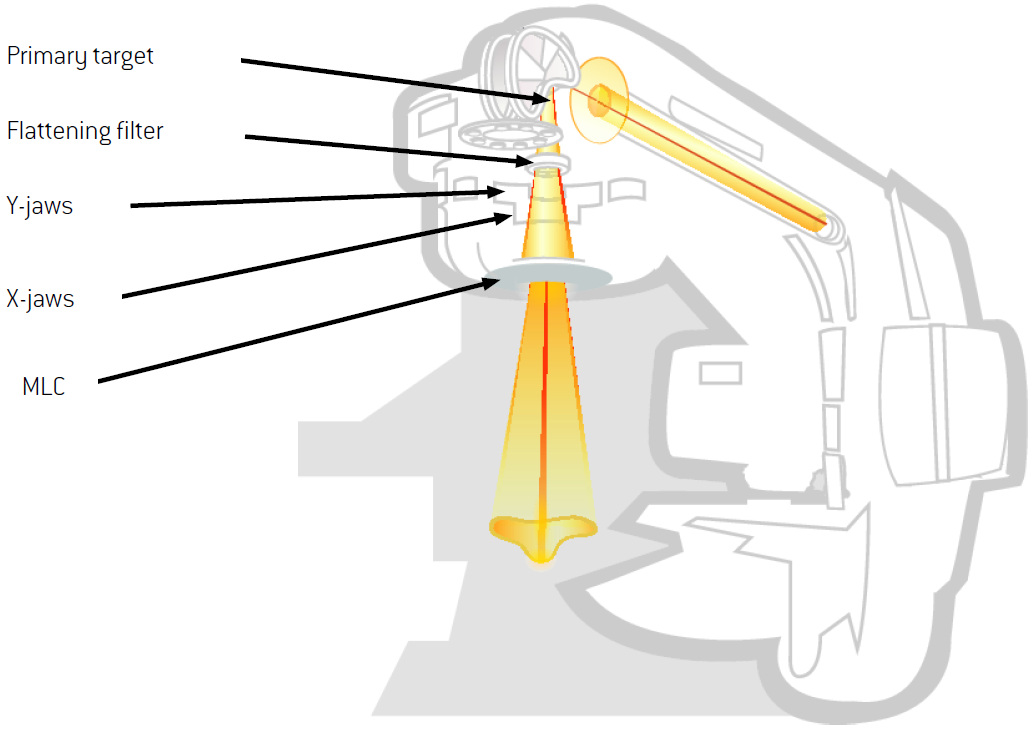
\includegraphics[width=.6\textwidth]{../cap1/linac.PNG}
\end{center}
\footnotesize
\structure{Radioterapia a fasci esterni:} tecnica medica che fa impiego di radiazioni ionizzanti per il trattamento di patologie (neoplasie maligne principalmente).\ac 
\structure{Dose fisica:} al pari della dose farmacologica è la quantità utilizzata per ottenere l'effetto terapeutico.
$$D = \frac{d \bar{\varepsilon}}{d m} \qquad\qquad \text{Unità: J\,kg}^{-1} \equiv \text{Gray [Gy]}$$
\end{frame}

\begin{frame}{Introduzione RT a fasci esterni}
\begin{center}
\small
\structure{Principali interazioni radiazione-paziente}\\ \vspace{.2cm}
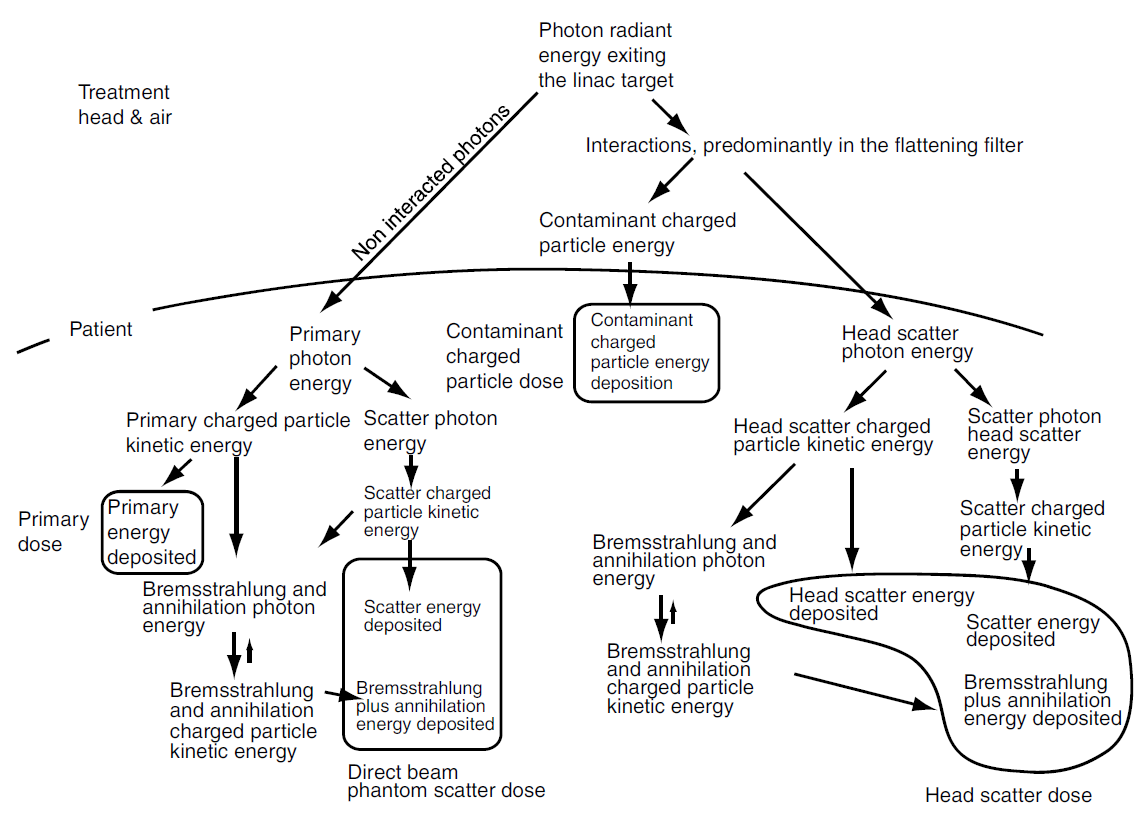
\includegraphics[width=.8\textwidth]{../cap1/processes.PNG}
\end{center}
\end{frame}



\begin{frame}{Introduzione RT a fasci esterni}
\begin{center}
\small
%\structure{Principali interazioni radiazione-paziente}\\ \vspace{.2cm}
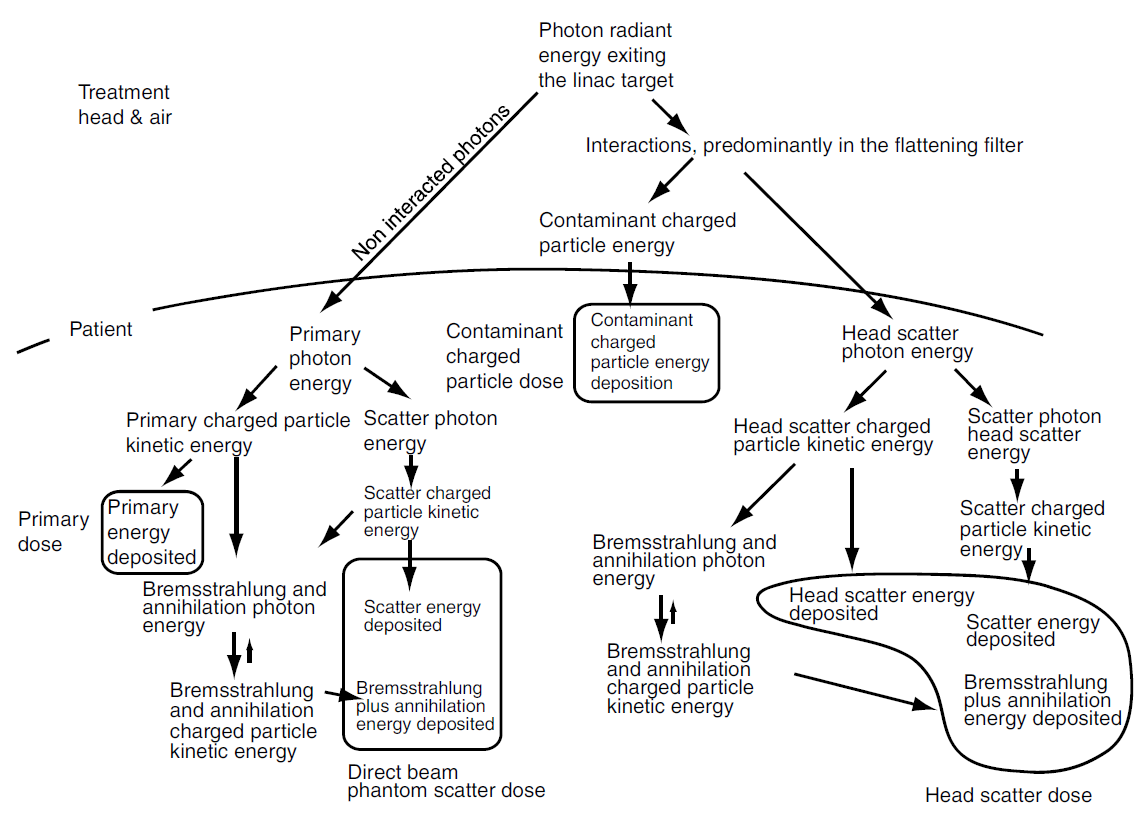
\includegraphics[width=.5\textwidth]{../cap1/processes.PNG}
\end{center}
\begin{itemize}
\footnotesize
\item \alert{Dose primaria:} originata dalla parte di fascio che non ha interagito nella testata $\Rightarrow$ $\sim 70\%$ della dose totale).
\item \alert{\textit{Head scatter dose}:} originata dalla parte di fascio che ha interagito nella testata (\textit{flattening filter}) $\Rightarrow$ $\sim 5\div 10\%$ della dose totale.
\item \alert{\textit{Phantom scatter dose}:} dovuta ai processi di scatter all'interno del paziente dalla parte di fascio che ha interagito nella testata (\textit{flattening filter}) $\Rightarrow$ $\sim 30\%$ della dose totale.
\item \alert{Dose da contaminazione:} originata dalla parte di fascio non fotonica (prevalentemente elettroni) $\Rightarrow$ comparabile con la dose primaria solo nei primi $mm$ di tessuto.
\end{itemize}
\end{frame}


\begin{frame}{Algoritmi di calcolo della dose}
\begin{columns}

\end{columns}
\end{frame}



\section[Modellizzazione del LINAC]{Modellizzazione fisica del LINAC nel TPS RayStation}
\begin{frame}{Indice}
\tableofcontents[currentsection]
\end{frame}

\begin{frame}{bla bla}
bla bla
\end{frame}

\section[La radioterapia adattiva]{La radioterapia adattiva, implementazione iniziale e sviluppi futuri}
\begin{frame}{Indice}
\tableofcontents[currentsection]
\end{frame}

\begin{frame}{bla bla}
bla bla
\end{frame}

\end{document}